\chapter{Results and performance}

\begin{figure}
    \begin{center}
    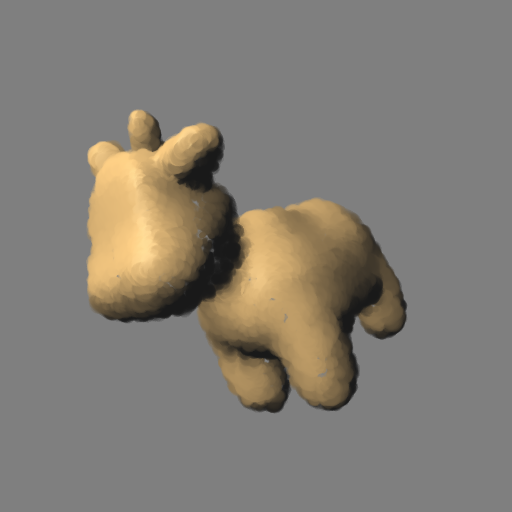
\includegraphics[width=50mm, height=50mm]{Resultats/spotPoint/final.png}
    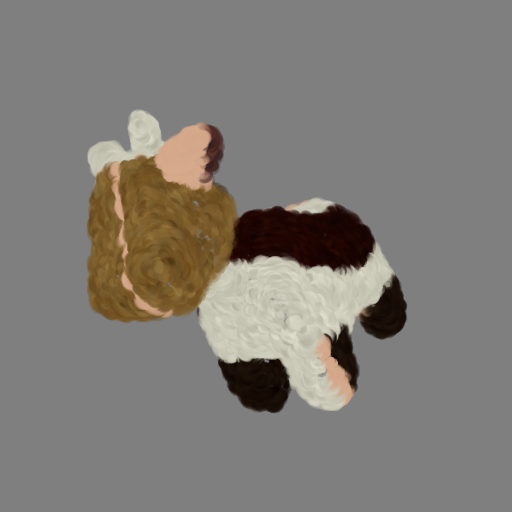
\includegraphics[width=50mm, height=50mm]{Resultats/spotPoint/final2.png}
    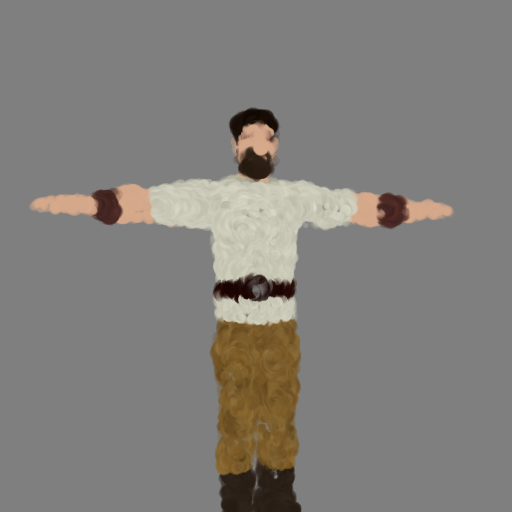
\includegraphics[width=50mm, height=50mm]{Resultats/pointCharacter/final.png}
    \end{center}
    \caption{Results of pointillism.}
    \label{results_point}
\end{figure}

\begin{figure}
    \begin{center}
    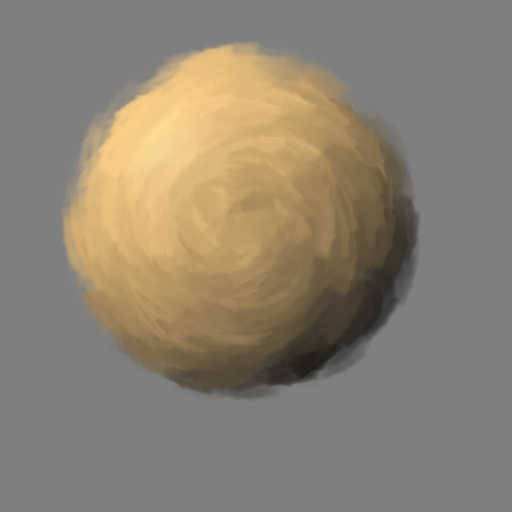
\includegraphics[width=50mm, height=50mm]{Resultats/painting1/final.png}
    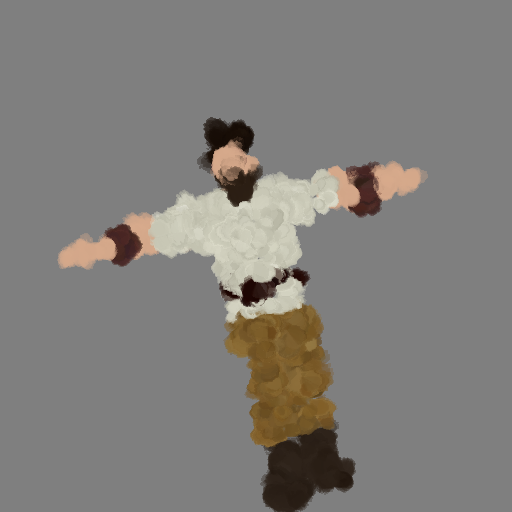
\includegraphics[width=50mm, height=50mm]{Resultats/paintChar/final.png}
    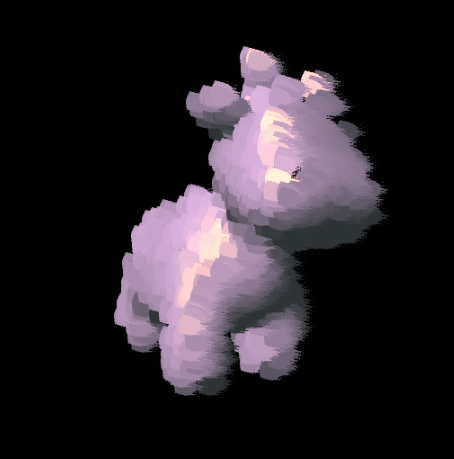
\includegraphics[width=50mm, height=50mm]{Resultats/spotPaint.png}
    \end{center}
    \caption{Results of brush painting.}
    \label{results_paint}
\end{figure}

\begin{figure}
    \begin{center}
    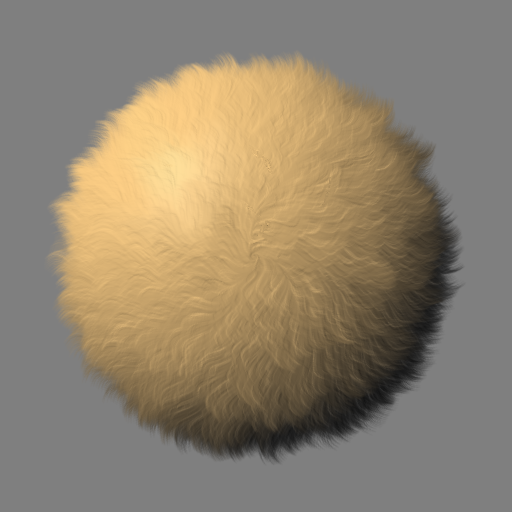
\includegraphics[width=50mm, height=50mm]{Resultats/bouledepoil1/final.png}
    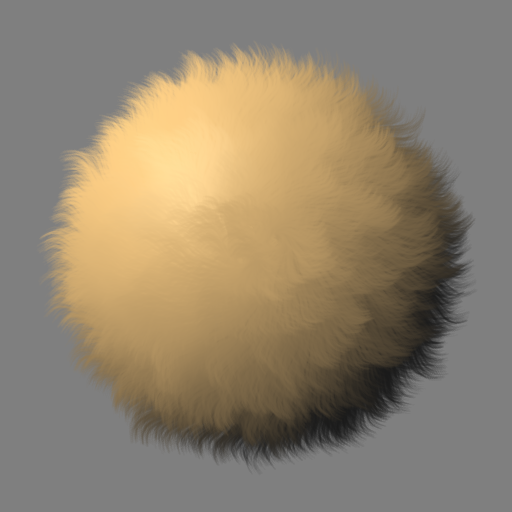
\includegraphics[width=50mm, height=50mm]{Resultats/bouledepoil2/final.png}
    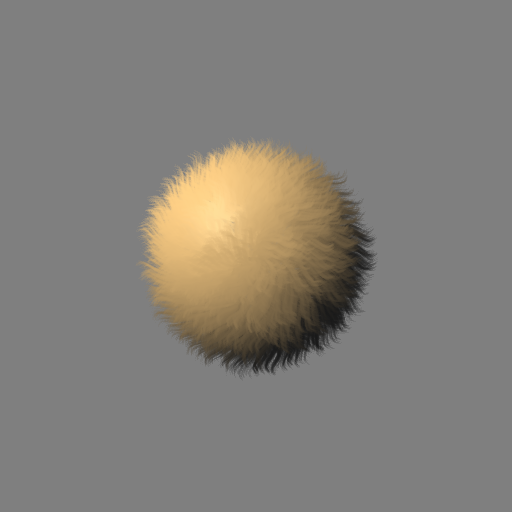
\includegraphics[width=50mm, height=50mm]{Resultats/bouledepoilFractalized/final.png}
    \end{center}
    \caption{Results of hairs rendering.}
    \label{results_hairs}
\end{figure}


Here there are some results of our method of stylization. The figure \ref{results_point} show some rendering with a point as mark and with differents color and models. We use the dot splat (the first in the figure \ref{splat_examples}) with a small size in order to keep a good level of details. In the figure \ref{results_paint} we tried to stylized as painted with brushes so we used brushe stroke as splat. In the figure \ref{results_hairs}, we tried to render hairs with our technique we a simple hair as splat. We rotated it according to the normals and to increase the realism we changed the size of the splat depending of a procedural noise to have in some areas of the object smaller splat and in some others areas bigger splat.





%%%% results
% several example with differents splats
% use noise to change the size of the splats in the object
% use tangents/normals map to rotate the splats
% differents shading



%%%% PERF
% nom de la carte
% resolution de l'image
% non-optimized
